El problema de síntesis de controlador ya tiene una solución clásica, por lo que la dificultad del trabajo no consistió en desarrollar un algoritmo que detectara estados ganadores y perdedores de un LTS totalmente explorado. 

El conflicto reside en que al componer distintos DES, la cantidad de estados de la composición es exponencial respecto de los estados en los componentes. Esto es de suma relevancia ya que la solución clásica, que compone toda la planta para luego explorarla, tiene un límite de escalabilidad en el cual la composición de la planta llega al límite de tiempo o memoria, y nunca se llega a la exploración.

Para combatir esto, la exploración on-the-fly, presentada en \cite{tesisDani}, clasifica estados como ganadores o perdedores durante la composición. Se espera que con esto sea posible, en primer lugar, cortar la exploración de una rama de la planta que ya se sabe que es perdedora o ganadora, reduciendo así la memoria y tiempo necesarios. Pero más aún, si el estado inicial fuera marcado como ganador o perdedor antes de la composición completa de la planta, ni siquiera sería necesario completar el proceso de composición.

En el listing \ref{lst:basic_on-the-fly} mostramos la estructura básica de este método. Trabajando sobre la parte de la planta compuesta hasta el momento (estructura explorada, $\structure$), se expande $\structure$ consiguiendo nueva información hasta que sea seguro si el estado inicial es ganador o perdedor en $E$. Al llegar a esta conclusión se retorna el controlador para $\initial$ en $E$ o se notifica que no es controlable.

\begin{definition}
	[Exploración Parcial] \label{def:unexploredTo}
	Sea $E = (S_E,$ $A_E, \D_E, \init{e}, M_E)$. Decimos que $ES$ es una exploración parcial de $E$ ($ES \subseteq E$) si $S_\structure \subseteq 
	S_E$ y $\structure = (S_\structure,A_E, \D_\structure,\init{e},M_E 
	\cap S_\structure)$, donde $ \D_\structure \subseteq (\D_E \cap 
	(S_\structure \times A_E \times S_\structure))$. Escribimos $ES \subset E$ cuando $S_\structure \subset S_E$.
\end{definition}

\begin{lstlisting}[language={pseudocode},label={lst:basic_on-the-fly},caption={Algoritmo on-the-fly básico},float=ht]
Algorithm basicOTF-Exploration($E, A_E^C$):
  $\initial$ = $\<\init{e}^0,\ldots,\init{e}^n\>$
  $\structure = (S_\structure,A_E, \D_\structure,\init{e},M_E 
  \cap S_\structure) \ldot ES \subseteq E$
  until surelyWinsOrLoses($\initial$):
    expandES()
    computeNewWinnersAndLosers($\structure$)
  if $initial \in \Goals$:
    return buildController($\initial$)
  else:
    return "UNREALIZABLE" 
\end{lstlisting}

Puede haber muchas variantes de cada una de estas partes, cómo se expande, cómo se computan nuevos ganadores y perdedores, etc. En particular, nuestro enfoque se muestra en el listing \ref{lst:on-the-fly} y consiste en ir agregando una transición a la vez a la parte conocida de la planta, y en cada paso ver si esta nueva transición permite concluir que un estado es ganador o perdedor. Si algún nuevo estado se clasifica como ganador  o perdedor, se propaga esta información a sus antecesores, posiblemente marcándolos a su vez como ganadores o perdedores, respectivamente.

A medida que exploramos mantenemos dos conjuntos de estados de $\structure$ ($\Goals$ y $\Errors$) para los cuáles ya se tiene una conclusión, es decir, se sabe que son ganadores (o perdedores) en $E$.

Como se demostrará en el capítulo \ref{chpt:dcs}, al expandir $\structure$ con una transición a la vez $(e,\l,e')$, a menos que $e'$ ya fuera un ganador/perdedor entonces solo puede haber nueva información si existe un loop entre $e$ y $e'$. Es más, si hay un nuevo estado ganador/perdedor, entonces $e$ seguramente es también un nuevo ganador/perdedor, y todos los nuevos estados clasificados son antecesores de $e$. Ésto permite optimizar la detección de nuevos ganadores/perdedores en lugar de ejecutar un algoritmo clásico sobre todo $\structure$.




Para explicar el algoritmo y argumentar su correctitud y completitud introducimos dos nuevos problemas de control para exploraciones parciales. Uno toma una visión optimista de la región no explorada ($\top$) asumiendo que todas las transiciones no exploradas llevan a un estado ganador. El otro toma una visión pesimista ($\bot$) asumiendo que las transiciones no exploradas llevan a estados perdedores.

\begin{definition}
	[Problemas de Control $\top$ y $\bot$] \label{def:unexploredTo}
	
	Sean $\E = (E, A_E^C)$, $E = (S_E,A_E,\D_E,\init{e},M_E)$ y $\structure = 
	(S_\structure,A_E, \D_\structure,\init{e},M_E \cap S_\structure)$, y $\structure 
	\subseteq E$.
	\\
	Definimos $\E_\top$ como $(\unexploredToTop{\structure}, A_E^C)$ donde 
	$\unexploredToTop{\structure} = (S_\structure \cup \, \{\top\},A_E,\D_\top, 
	\init{e}, 
	(M_E \cap S_\structure)\, \cup \, \{\top\})$ y $\, \D_\top \, = \, \D_\structure 
	\, 
	\cup\, \{(s,\l, \top) 
	\;$ $ | \; \exists s' \ldot (s, \l, s') \in (\D_E \setminus \D_\structure)\} \cup \{(\top, \l, \top) \, | \, \l \in A_E\}$ \\
	Definimos $\E_\bot$ como $(\unexploredToBottom{\structure}, A_E^C)$ donde 
	$\unexploredToBottom{\structure} = (S_\structure \, \cup \, 
	\{\bot\},A_E,\D_\bot, 
	\init{e}, M_E \cap S_\structure)$ y $\D_\bot = \D_\structure \, \cup \, \{(s,\l, 
	\bot) \, | \, $ $ \exists s' \ldot (s, \l, s') \in (\D_E \setminus \D_\structure)\}$ 
\end{definition}

Usamos estos problemas de control para decidir tempranamente si un estado $s$ es ganador o perdedor en $E$ basado en lo que exploramos previamente en $\structure$. Si $s$ es ganador en $\unexploredToBottom{\structure}$ esto significa que sin importar a dónde lleven las transiciones no exploradas, $s$ también va a ser ganador en $E$. Similarmente, $s$ es perdedor en $E$ si es perdedor en $\unexploredToTop{\structure}$.
El Lema~\ref{lem:WESandLesMonotonicity} refuerza este razonamiento.


\begin{lemma}\textbf{\emph{(Monotonicidad de $\WES$ y $\LES$)}}
	\label{lem:WESandLesMonotonicity}
	Sean $\structure$ y $\structure'$ dos exploraciones parciales de $E$ tal que $\structure 
	\subset \structure'$ entonces $\WES \subseteq \WESS$ y $\LES \subseteq 
	\LESS$.
\end{lemma}

El algoritmo agrega iterativamente una transición de $E$ a $\structure$ a la vez y asegura que al final de cada iteración, los estados en $\structure$ están correcta y completamente clasificados en ganadores y perdedores si hay suficiente información de $E$ en $\structure$. Los conjuntos de estados $Errors$, 
$Goals$ y $\NONE$ se usan para este propósito.



En el peor caso, si no se pudo concluir nada antes de componer la planta en su totalidad, se perdió tiempo en los puntos fijos, intentando clasificar estados, y se realiza una última vez el algoritmo clásico con la planta totalmente explorada. Esto garantiza la completitud del algoritmo, como se detalla en mayor profundidad en el capítulo~\ref{chpt:dcs}.

\begin{lstlisting}[language={pseudocode},label={lst:on-the-fly},caption={Nuestro enfoque on-the-fly},float=ht]
Algorithm genericOTF-Exploration($E, A_E^C$):
   $\initial$ = $\<\init{e}^0,\ldots,\init{e}^n\>$
   $\Goals = \Errors = \emptyset$
   $\structure = initial$ //la parte conocida de la planta
   while $initial \notin \Goals \cup \Errors$:
     $(e,\l,e') = $nextTransition($\structure, heuristica$)
     expandES($\structure,(e,\l,e')$)
     if $e' \in \Errors$:
       propagateError($e'$)
     else if $e' \in \Goals$:
       propagateGoal($e'$)
     else if isLoop($e,e'$):
       if newWinningLoop($e,e'$):
         propagateGoal($e'$)
       else if newLosingLoop($e,e'$):
         propagateError($e'$)
         
   if $initial \in \Goals$:
     return buildController($\Goals$)
   else:
     return "UNREALIZABLE"  
\end{lstlisting}

Para explorar en el orden más conveniente, y componer una menor parte de la planta, se utiliza una heurística de exploración Best First Search \cite{tesisDani}. La misma busca ganar controlablemente o perder no controlablemente, para garantizar con la menor exploración posible que el estado actual es ganador o perdedor.

Una heurística no presenta garantía de resultados perfectos, más bien da una recomendación. Son ampliamante utilizadas al optimizar, pero es importante que la correctitud de los algoritmos no dependan de estas recomendaciones, ya que por su misma naturaleza no tienen garantías fuertes.

\section{Agnosticismo a la heurística}

Una distinción clave del algoritmo \textit{on-the-fly} es que está dividido en dos partes. Por un lado se tiene el algoritmo de exploración responsable de que al final se llegue al resultado correcto, por el otro tenemos una heurística que le brinda la próxima transición a explorar. Ese algoritmo de exploración no puede depender de la heurística, ya que la misma no garantiza siempre elegir el mejor camino posible, sino solo la mejor aproximación que encuentre. Uno de los focos de nuestro trabajo fue en esa corrección independiente del orden de exploración de las transiciones.

El proyecto \texttt{MTSA} inicialmente contaba con dos heurísticas \texttt{Best First Search} para exploración, \textit{Monotonic Abstraction} y \textit{Ready Abstraction}. 

El inconveniente con la versión anterior del algoritmo de exploración es que había sido desarrollado en conjunto con las heurísticas. Si bien esto ayudaba a la eficiencia del mismo, generaba una dependencia del orden de observación de las transiciones, dando resultados erróneos al cambiar las recomendaciones. El nuevo enfoque no depende de la forma de explorar, por ende, da una mayor libertad de investigar a futuro nuevos criterios de evaluación para mejorar la eficiencia de la técnica sin comprometer corrección ni completitud. Esto fue útil durante el desarrollo del trabajo, ya que facilitó la inclusión de nuestras nuevas heurísticas (\texttt{Dummy} y \texttt{Breadth First Search}, ver sección \ref{chpt:heurist-nuevas}) para la experimentación.


\section{Ejemplo de ejecución}

Para ilustrar el funcionamiento y ventajas de la exploración on-the-fly, mostramos una ejecución posible sobre una planta ejemplo. Supongamos que dados ciertos autómatas calculamos su composición y llegamos a la planta de la figura \ref{fig:ej:plantaCompleta}. Las transiciones se van a explorar en orden de menor a mayor, en el diagrama las (u)/(c) son no controlables/controlables respectivamente y el estado marcado tiene doble círculo. No especificamos la controlabilidad de todas las transiciones de manera de hacer más legible el gráfico y además porque, mirando las definidas, no nos modifica la conclusión el hecho de que sean o no controlables. %TODO ok esto no? es confuso? lo sacamos?  

\begin{figure}
 \centering
 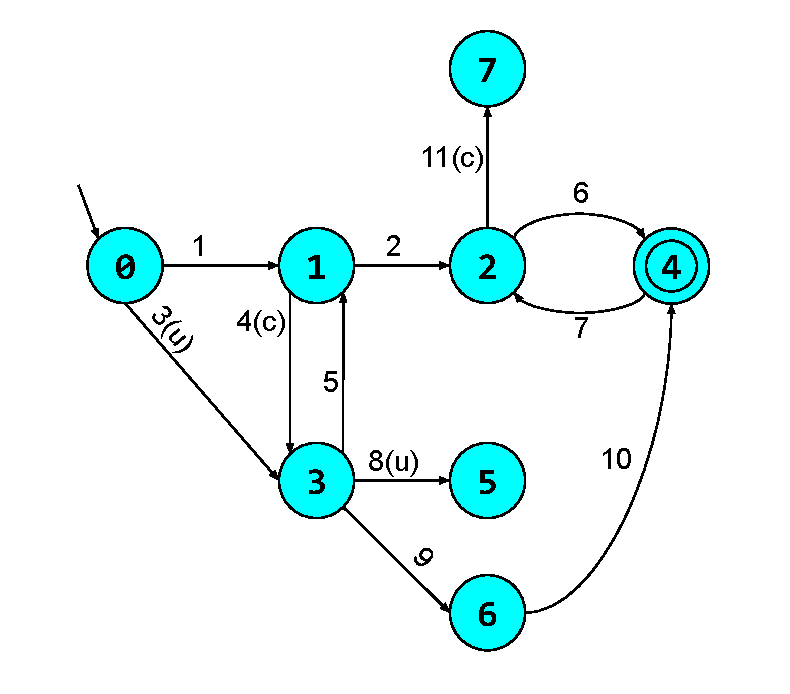
\includegraphics[scale=0.6]{figures/ejemplo_on-the-fly/0.pdf}
 \caption{Planta compuesta completa}
 \label{fig:ej:plantaCompleta}
\end{figure}

Al iniciar el algoritmo no vemos la planta completa sino sólo el primer estado \cyan{0}, desde el mismo expandimos la primer transición, en este caso \textit{1}. Como llega a un estado sin explorar \cyan{1}, y que no es deadlock, no hay información para conseguir. Entonces mientras lleguemos a ``algo nuevo'' no tenemos nada para hacer más que seguir explorando.
Incluso si llegamos a un estado explorado (no deadlock) no va a haber nueva información si no tenemos un loop. Veremos más en detalle y con demostración por qué esto es así en el capítulo \ref{chpt:dcs}; pero la intuición es que no va a haber nuevos ganadores puesto que un ganador necesita llegar a un marcado infinitas veces, por ende necesita como mínimo que haya un loop. Entonces hasta ahora llevamos explorado lo mostrado en la figura \ref{fig:ej:exploracion1}.

\begin{figure}[h]
 \centering
 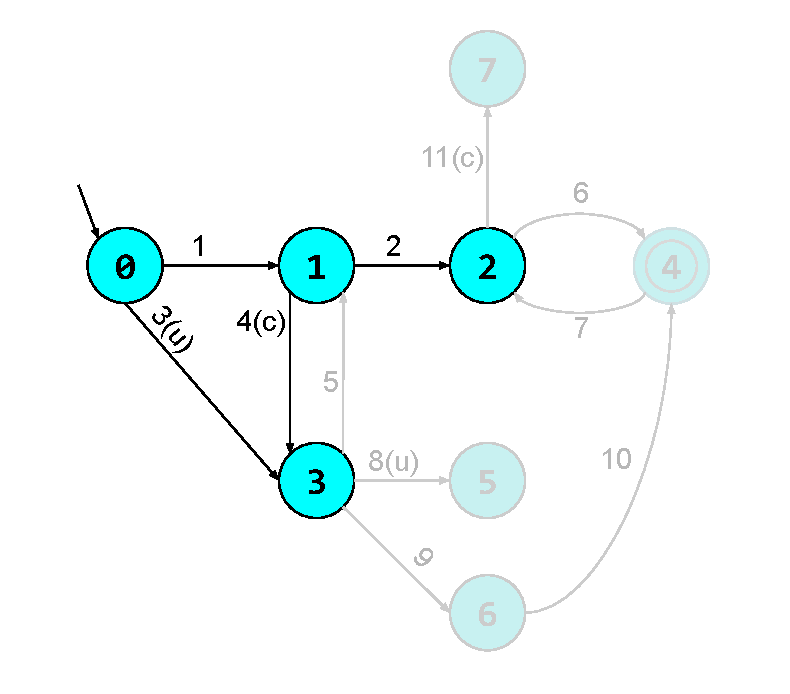
\includegraphics[scale=0.6]{figures/ejemplo_on-the-fly/1.pdf}
 \caption{Primeros pasos de exploración}
 \label{fig:ej:exploracion1}
\end{figure}

Si seguimos explorando por la transición \textit{5} cerramos un loop [\cyan{1}, \cyan{3}], pero \cyan{3} puede ser forzado a algo no explorado usando la transición no controlable \textit{8}, entonces todavía no podemos sacar conclusión alguna. Exploramos hasta figura \ref{fig:ej:exploracion2}.

\begin{figure}
 \centering
 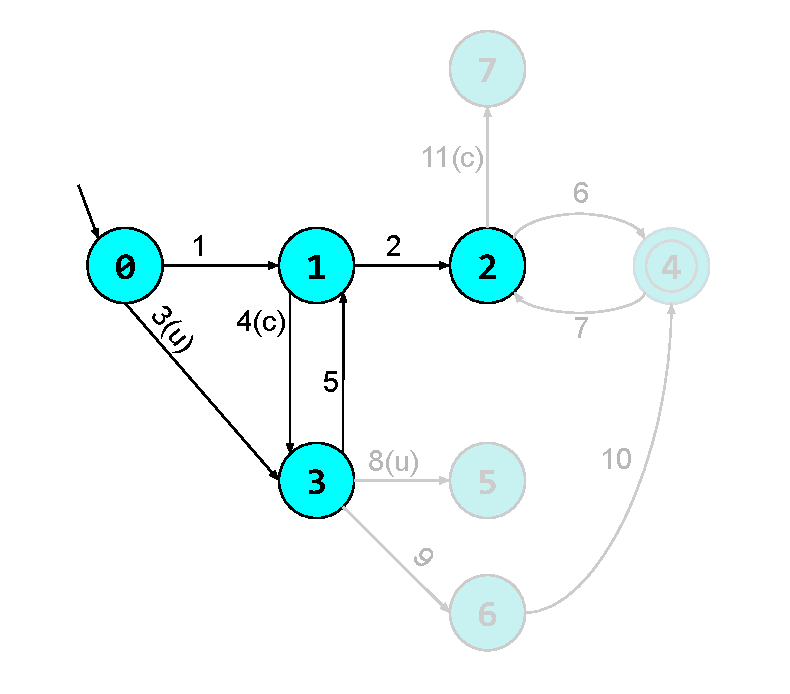
\includegraphics[scale=0.6]{figures/ejemplo_on-the-fly/2.pdf}
 \caption{Hay loop sin conclusiones nuevas}
 \label{fig:ej:exploracion2}
\end{figure}

Continuamos y llegamos a un estado marcado \cyan{4}, si fuese sólo alcanzar un marcado podríamos decir que es ganador pero necesitamos siempre poder llegar a uno (incluso desde sí mismo), por ende ahora sigue sin ser nada. Luego vemos \textit{7}, cerrando loop [\cyan{2}, \cyan{4}]. Éste loop tiene un estado marcado y \cyan{2} no puede ser forzado a otra cosa, ya que el resto de sus transiciones son controlables; por ende obtenemos nuestros primeros ganadores (\cyan{2} y \cyan{4}). A continuación debemos propagar esta nueva información llegando a marcar \cyan{1} como ganador, porque puede controlablemente llegar al loop [\cyan{2}, \cyan{4}]. Lamentablemente todavía no hay conclusión sobre el estado inicial debido a que puede ser forzado a algo sin explorar. Ver figura \ref{fig:ej:exploracion3}.

\begin{figure}[h]
 \centering
 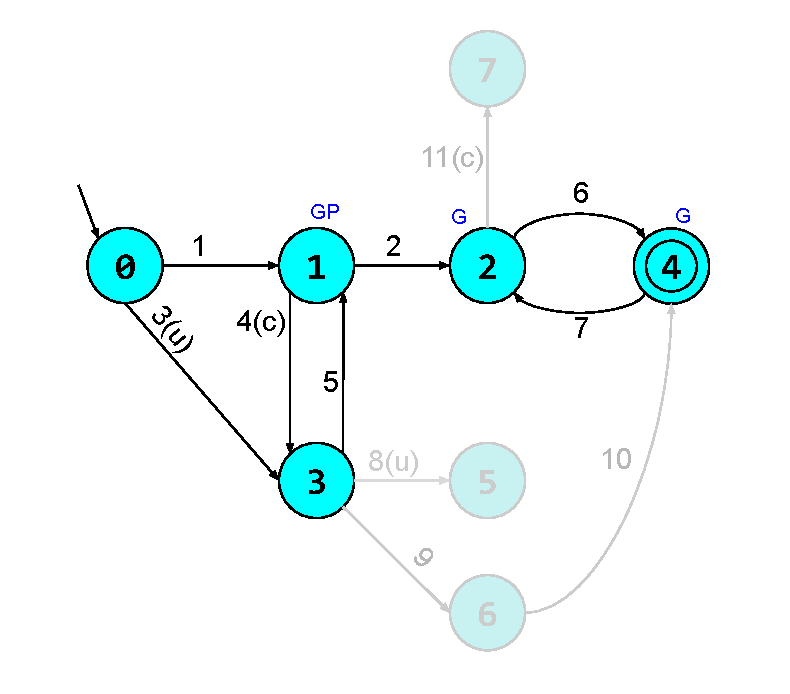
\includegraphics[scale=0.6]{figures/ejemplo_on-the-fly/3.pdf}
 \caption{Se encuentra Goal [2, 4] y propaga (1)}
 \label{fig:ej:exploracion3}
\end{figure}

Proseguimos con \textit{8} y llegamos a explorar el estado \cyan{5}, que es un deadlock por ende es error directamente. Propagando esta información marcamos los estados \cyan{3} y \cyan{0} como errores, llegando así a una conclusión sobre el inicial. Entonces ya no nos es necesario seguir explorando y se retorna que \textit{no existe controlador para la planta}. El estado de exploración final de la planta se ve en la figura \ref{fig:ej:exploracion4}.

\begin{figure}
 \centering
 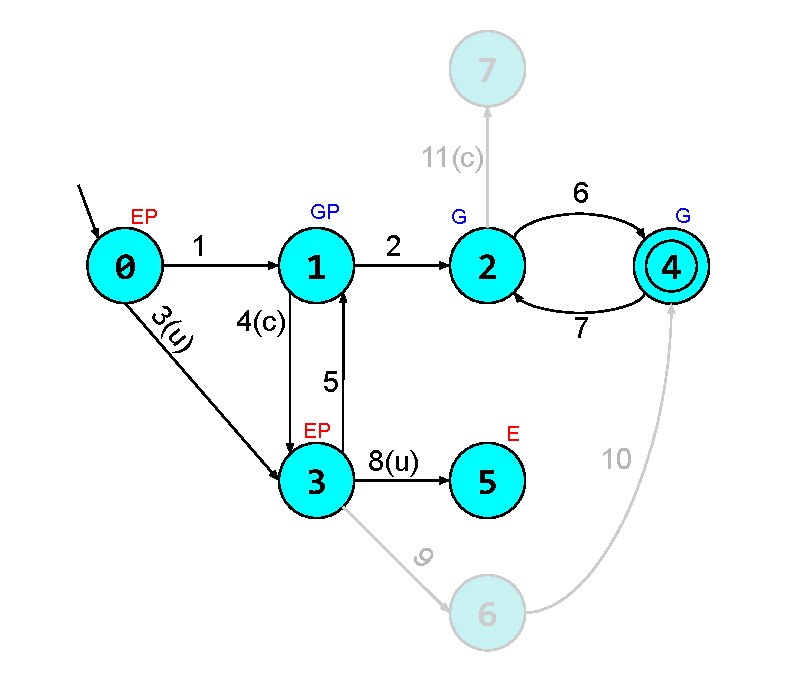
\includegraphics[scale=0.6]{figures/ejemplo_on-the-fly/4.pdf}
 \caption{Se encuentra Error (5) y propaga hasta inicial (3, 0), dejando de explorar}
 \label{fig:ej:exploracion4}
\end{figure}

Notar que no vemos las demás transiciones de \cyan{2} ni \cyan{3} ya que, en el caso de \cyan{2} gana por alguna y el resto son controlables, y en el caso de \cyan{3} pierde por una no controlable. Es decir, \cyan{2} puede controlablemente ganar y \cyan{3} es forzado a perder sin importar la forma del resto.

Observación opcional: Si la transición \textit{8} fuese controlable podríamos evitar el error y seguiríamos explorando, encontrando el estado \cyan{6}, su conexión al loop ganador y propagando ganador hasta el estado inicial. Notar que ésta sería una planta \textit{diferente}, controlable a diferencia de la propuesta en el ejemplo.












%\section{Invariante}\label{sct:invariante}

%Intentando resolver el problema del marcado explícito de errores, buscamos una separación fuerte entre los estados $error \in L_E$ y los estados para los cuales no tenemos suficiente información para clasificar en este momento $\NONE$. Para esto, los lemas detallados en la sección de demostración del algoritmo aseguran que un estado marcado como ganador o perdedor lo es en la planta compuesta totalmente explorada, y nunca puede cambiar su estado.

%Como se verá en la propiedad~\ref{def:invariant} del siguiente capítulo, un estado $s$ solo puede seguir sin clasificar (siendo $\NONE$) si, con los explorados hasta el momento, y siendo totalmente optimistas sobre las transiciones desconocidas no podemos asegurar que $s$ está condenado a ser perdedor (y tampoco podemos concluir que es ganador siendo pesimistas).

%Al momento de haber explorado todos los descendientes de $s$, incluso si no se exploró toda la planta total, es claro que no importa si se es optimista ($\top$) o pesimista ($\bot$) para saber si $s$ es un estado ganador o perdedor, por lo que nos forzamos por nuestro invariante a clasificarlo. Con esto evitamos las ramas totalmente exploradas pero sin clasificar que traían complicaciones en la figura~\ref{fig:falenciasErrores} y solo permitimos que un estado sea $\NONE$ si tiene un camino a una transición no explorada.\\



